%%%%%%%%%%%%%%%%%%%%%%%%%%%%%%%%%%%%%%%%%
% Stylish Article
% LaTeX Template
% Version 2.2 (2020-10-22)
%
% This template has been downloaded from:
% http://www.LaTeXTemplates.com
%
% Original author:
% Mathias Legrand (legrand.mathias@gmail.com) 
% With extensive modifications by:
% Vel (vel@latextemplates.com)
%
% License:
% CC BY-NC-SA 3.0 (http://creativecommons.org/licenses/by-nc-sa/3.0/)
%
%%%%%%%%%%%%%%%%%%%%%%%%%%%%%%%%%%%%%%%%%

%----------------------------------------------------------------------------------------
%	PACKAGES AND OTHER DOCUMENT CONFIGURATIONS
%----------------------------------------------------------------------------------------

\documentclass[fleqn,10pt]{SelfArx} % Document font size and equations flushed left

\usepackage[english]{babel} % Specify a different language here - english by default
\usepackage{lipsum} % Required to insert dummy text. To be removed otherwise
\usepackage{csquotes}
\usepackage[makeroom]{cancel}
\usepackage[sorting=none, style=nature]{biblatex}
\bibliography{bibliography.bib}

\graphicspath{{./Figures/}}
%----------------------------------------------------------------------------------------
%	COLUMNS
%----------------------------------------------------------------------------------------

\setlength{\columnsep}{0.55cm} % Distance between the two columns of text
\setlength{\fboxrule}{0.75pt} % Width of the border around the abstract

%----------------------------------------------------------------------------------------
%	COLORS
%----------------------------------------------------------------------------------------

\definecolor{color1}{RGB}{39,104,13} % Color of the article title and sections
\definecolor{color2}{RGB}{222,121,32} % Color of the boxes behind the abstract and headings

%----------------------------------------------------------------------------------------
%	HYPERLINKS
%----------------------------------------------------------------------------------------

\usepackage{hyperref} % Required for hyperlinks

\hypersetup{hidelinks,
	colorlinks,
	breaklinks=true,
	urlcolor=color2,
	citecolor=color1,
	linkcolor=color1,
	bookmarksopen=false,
	pdftitle={Title},
	pdfauthor={Author},
	}

%----------------------------------------------------------------------------------------
%	ARTICLE INFORMATION
%----------------------------------------------------------------------------------------

\JournalInfo{Academic Year 2022-2023} % Journal information
\Archive{Network Modeling and Simulation [146100] - prof. L. Marchetti} % Additional notes (e.g. copyright, DOI, review/research article)

\PaperTitle{Validation of a Mathematical Model Describing the Dynamics of Chemotherapy for Chronic Lymphocytic Leukemia In Vivo} % Article title

\Authors{Alessia Guadagnin Pattaro\textsuperscript{1}, Giovanni Plazzotta\textsuperscript{1}, Annarita Zanon\textsuperscript{1}} % Authors
\affiliation{\textsuperscript{1}\textit{Master's degree in Quantitative and Computational Biology, University of Trento}} % Author affiliation

%\Keywords{Keyword1 --- Keyword2 --- Keyword3} % Keywords - if you don't want any simply remove all the text between the curly brackets
%\newcommand{\keywordname}{Keywords} % Defines the keywords heading name

%----------------------------------------------------------------------------------------
%	ABSTRACT
%----------------------------------------------------------------------------------------

\Abstract{To be added}

%----------------------------------------------------------------------------------------

\begin{document}

\maketitle % Output the title and abstract box

%\tableofcontents % Output the contents section

\thispagestyle{empty} % Removes page numbering from the first page

%----------------------------------------------------------------------------------------
%	ARTICLE CONTENTS
%----------------------------------------------------------------------------------------

\section{Introduction} % The \section*{} command stops section numbering

%\addcontentsline{toc}{section}{Introduction} % Adds this section to the table of contents

\subsection{Chronic Lymphocytic Leukemia}
The paper under analysis sets itself the aim of building a mathematical model able to describe the interaction between malignant chronic lymphocytic leukemia (CLL) cells, effector cells, which in the case of cancer response are mainly NK cells (innate immunity) and T CD8 lymphocytes (adaptive immunity), and two different drugs, the Bruton tyrosine kinase (BTK) inhibitor Ibrutinib (Ibr) and an inhibitor of the enzyme topoisomerase, Cytarabine (Cyt), whose introduction has transformed CLL therapy and contributed to extend the overall survival of patients. Additional details about these small - molecule drugs will be presented in the sections below. While the formulation of a mathematical model describing the dynamics of cancer in an immunoactive environment is not innovative \textit{per se}, this paper sets itself apart in the sense that:
\begin{itemize}
\item It deals with a blood cancer instead of a solid tumor: in blood cancers, cell growth, survival dynamics and cellular interactions within the
tumor microenvironment likely differ considerably from solid tumors. It is expected that several parameters of previusly formulated ODE - based computational models need to be adapted for blood-borne cancers.
\item The majority of models use data generated by simulations to perform the parameter estimation, instead of experimental data. This paper, on the other hand, is strongly experimentally - oriented.
\item Even when data are derived from experiments, these are often performed \textit{in vitro} rather than \textit{in vivo}, and many studies have demonstrated conflicting results, in particular for what concerns optimal drug doses, between these two approaches. This paper, on the other hand, describes \textit{in vivo} experiments, performed on murine models injected with A20 CLL cells, aimed at the estimation of the cancer cells growth rate $r$ and of the cytotoxicity rates $\mu_{AC}$ as a function of therapy. \par
\end{itemize}
\vspace{0.4cm}
Chronic lymphocytic leukemia (CLL) is the most common type of blood cancer in adults in the Western world, with an incidence of 4.9 cases in 100000 people per year. It typically occurs in elderly patients, with the median age at diagnosis being 70 years. CLL is characterized by the clonal proliferation and accumulation of mature B lymphocytes in secondary lymphoid organs, spleen, peripheral blood, and bone marrow. \cite{cll-burger-med, cll-rozman-med}  There is no known cause for this disease, but it is suspected to have a genetic component. Loss or addition of large chromosomal material followed by additional mutations, that render the leukemia increasingly aggressive, are often observed. Additionally, mutations in \textit{IGHV} (immunoglobulin heavy variable) genes distinguishing different types of clinical behaviours of CLL and are prognostic of patent outcome \cite{immunogl-med}. \par
%Treatment of Chronic Lymphocytic Leukemia - Burger Jan A.
%Chronic Lymphocytic Leukemia - Rozman et al
%Immunoglobulin heavy variable (IGHV) genes and alleles - Xochelli et al 
\vspace{0.4cm}
Different treatment strategies are available for patients suffering from CLL. It is important to notice that studies on early-stage disease were unable to show a benefit of early therapeutic interventions: treatment of patients with early stage CLL did not result in a survival benefit. For this reason, and not to fruitlessly trigger the development of drug resistance, patient in these stages should not be treated, but only monitored, until the disease becomes \textit{active}. The degree of \textit{activity} of CLL can be assessed using the following guidelines:
\begin{itemize}
    \item Progressive lymphocytosis with an increase of $\geq 50 \%$ over a 2 month period, or lymphocyte doubling time of less than 6 months.
    \item Worsening of anemia and/or thrombocytopenia
    \item Massive nodes (i.e., $\geq 10$ cm in longest diameter)
    \item Massive or symptomatic splenomegaly and hepatomegaly
    \item Autoimmune complications
    \item Functional extranodal involvement (e.g., skin, kidney, lung, spine)
    \item Significant weight loss and fatigue, fevers above 38 degrees for more than two weeks, night sweats. 
\end{itemize}
When the treatment becomes necessary, specialists can choose between different classes of drugs, targeting different aspects of the cellular structure (e.g. surface antibodies), metabolism and external microenvironment:
\begin{itemize}
\item Cytostatic agents: having the goal to stop cellular proliferation by interfering with the replication process. Examples are purine analogs, such as Cytarabine (Cyt), one of the two drugs that we will discuss in this presentation.
\item Monoclonal Antibodies: specifically built to interact with surface antigens that have been documented to be overexpressed in malignancies, like CD-20 and CD-52 receptors in B-cells blood cancers. They have the goal of guiding the immune system towards the cancerous cells. Examples are Rituximab and Alemtuzumab.
\item Signalling - targeting agents: having the goal of interfering with the embedded signalling pathways in order to trigger apoptosis. Ibrutinib (Ibr), the second drug discussed in this presentation, is a Bruton Tyrosine Kinase inhibitor that hinders the downstream propagation of the signal generated by bounded BCR receptors, stopping the activation of B cells survival pathways. 
\item Immunotherapy: different CART approaches are being explored.
\end{itemize} \par
\vspace{0.4cm}
Finally, a worth noting characteristics of CLL is its incurability, at least for the patients who do not undergo allogeneic stem cell transplantation. This is due to the very low level of clonality displayed by the majority of somatic \textit{"passenger"} mutations that accumulate above the background of \textit{"driver"} mutations that originally gave birth to the malignancy. A very low level of clonality implies a very high tumor heterogeneity, with different subpopulations carrying different sets of mutations, and in turn a very high tumor heterogeneity increases the probability of developing primary resistance. \par




%------------------------------------------------

\section{Materials and methods}
\subsection{Ibrutinib (Ibr)}
Ibrutinib (Ibr) is a chemotherapic drug (Fig. \ref{fig:Ibr}) used as a deactivator of Bruton tyrosine kinase (BTK). The pathogenesis of many lymphocytes-related malignancies \cite{ibr-1} involves aberrant behaviour of B cells receptor signalling, alongside antigen-dependent activation of BTK.\\
Ibr blocks B cell antigen receptor signalling through an irreversible covalent bond with Cys-481 of BTK, hence reducing malignant B cell proliferation and inducing cell death.\\
The drug reaches its maximum concentration in plasma ($953\,\text{ng}\cdot\text{h}/\text{mL}$ at a dosage of $560\,\text{mg}/\text{day}$) in 1-2 h and is widely distributed in the body. The major route of elimination is hepatic metabolism due to cytochrome P450 3A enzymes. It has an elimination half-life of 4-6 h via faeces.\\
Ibr has a high tolerance level in the body, clinical studies have shown that dose-limiting events are not observed even with prolonged dosing \cite{ibr-2} but the saturation of the active site of BTK was reached after a single dose of 2.5 to 20 mg/kg \cite{ibr-pubchem}. Reported dosages administered Ibr in 1.25, 2.5, 5.0, 8.3, 12.5, and 17.5 mg/kg/day for 28 days orally, with a 7-day rest period \cite{ibr-2}.
\begin{figure}[htbp!]
	\centering
	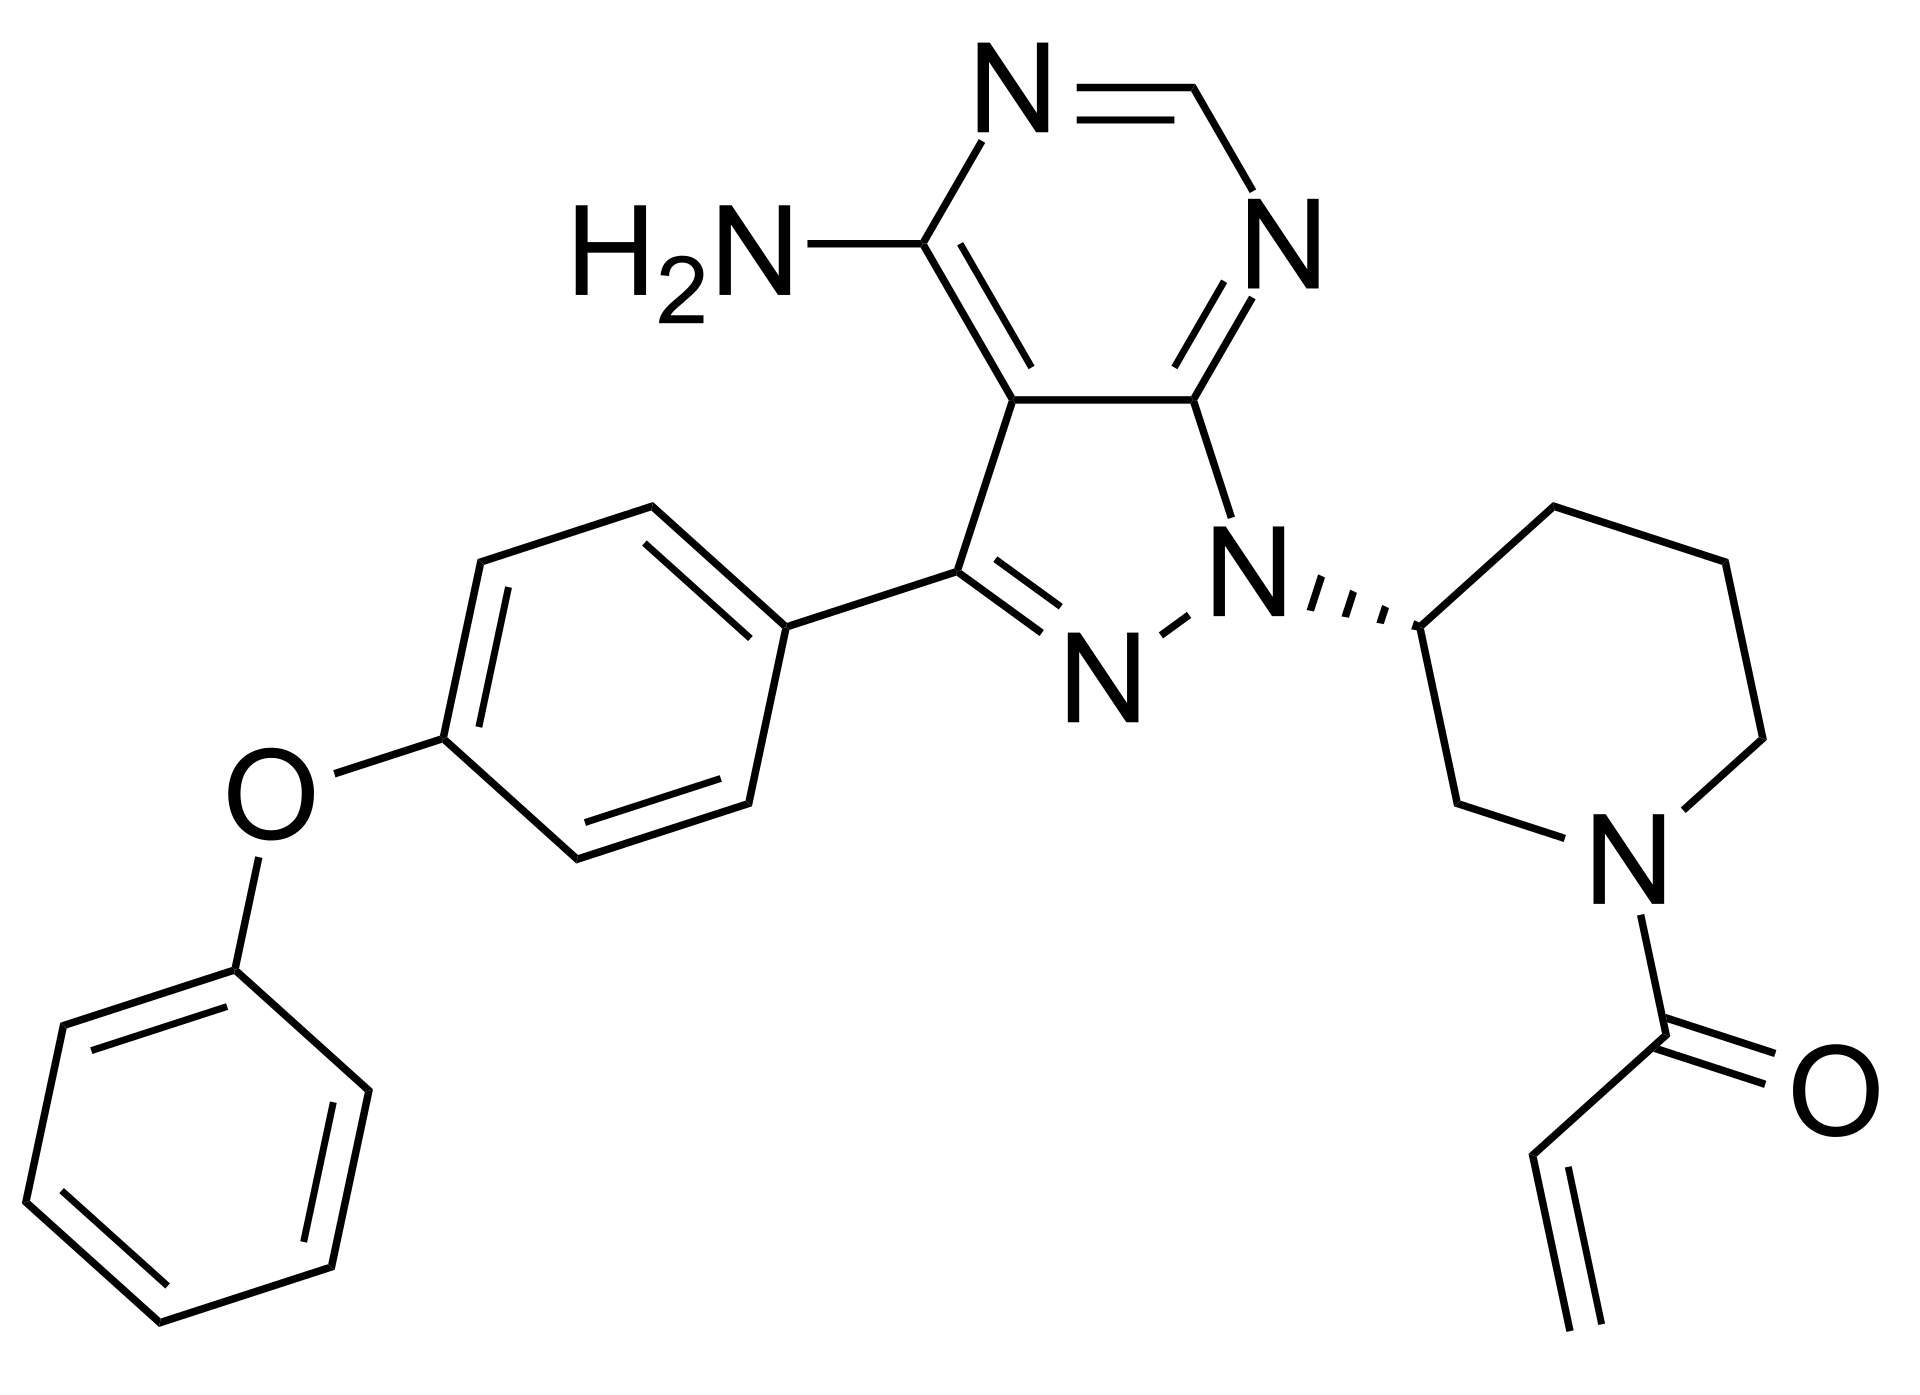
\includegraphics[scale=0.1]{Ibrutinib.png}
	\caption{Molecular structure of chemotherapeutic drug Ibrutinib}
	\label{fig:Ibr}
\end{figure}

%--------------------------
\subsection{Cytarabine (Cyt)}
Cytarabine (Cyt), also called arabinosylcytosine, is a medication used in the treatment of leukaemias and lymphomas that acts as an antimetabolite and antineoplastic. In Fig. \ref{fig:Cyt}, it can be seen that it is a nucleoside (pyrimidine analogue) with arabinose sugar.
The sugar moiety induces the rotation of Cyt within the DNA, blocking DNA replication during the S-phase of cellular replication. It also acts on DNA polymerase and its maximum effects are seen after the time equivalent to a full cell cycle (8-12 h). 
The drug is administered via intravenous infusion and it was shown that the dose-response relationship for Cyt has a plateau above a dose level of 1000 mg/$m^2$. The reported dosage for patients is a first cycle with 200 mg/$m^2$ of Cyt infused continuously for 24 hours, and a second cycle with 1000 mg/$m^2$ infused for three hours twice a day \cite{cyt-3}.
Cyt has two types of metabolites: 
\begin{itemize}
	\item \textbf{inactive metabolites}, from deamination as soon as the drug enters the plasma
	\item \textbf{active metabolites} (Cyt triphosphate, CytTP), after being transported into the cell, and after phosphorylation.
\end{itemize}
The active metabolites competitively inhibit DNA polymerase, they are incorporated into DNA where they act as chain terminators, leading to incomplete DNA replication and cell death.\\
CytTP has a saturation level, leading to accumulation of the metabolite in cells, a lower drug selectivity of cancer cells, and a higher degree of myelosuppression\cite{cyt-1, cyt-2}.
\begin{figure}[htbp!]
	\centering
	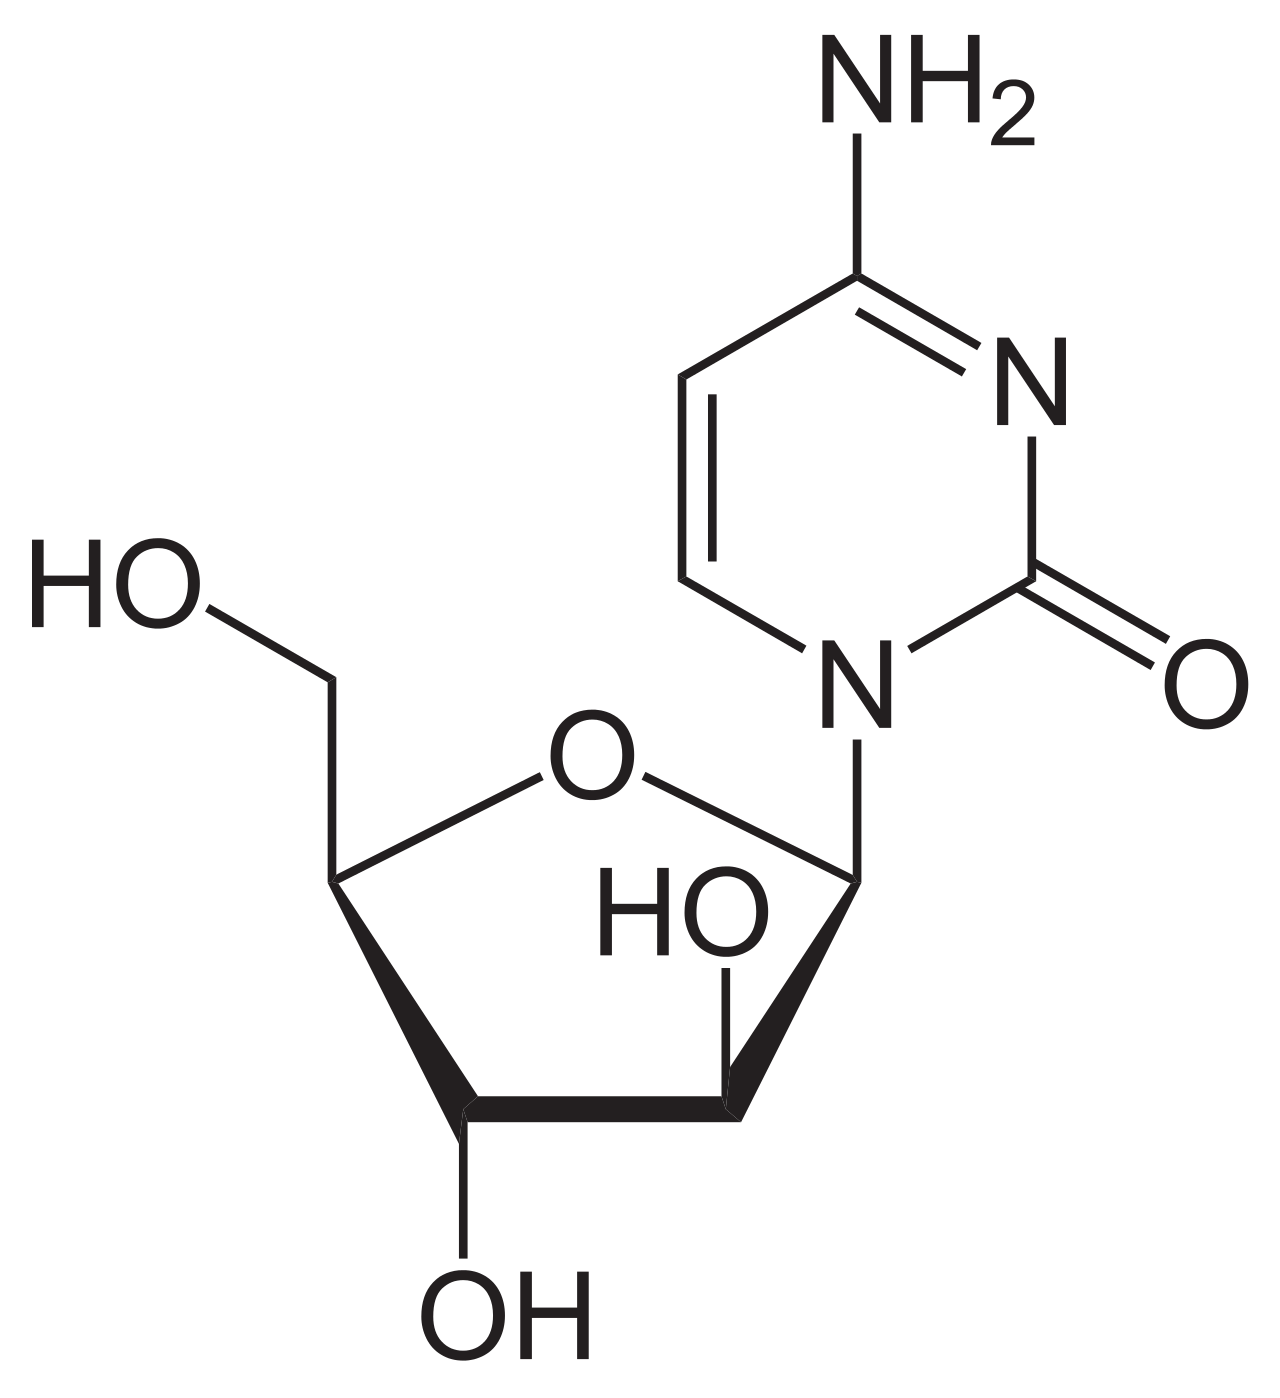
\includegraphics[scale=0.1]{Cytarabin.png}
	\caption{Molecular structure of chemotherapeutic drug Cytarabine}
	\label{fig:Cyt}
\end{figure}




%------------------------------------------------

\section{Paper analysis}
\subsection{Mathematical model}
Based on previous studies, an ODE model was formulated to explain the interaction between CLL cells, immune cells and chemotherapeutic drugs:

\[
\begin{cases} 
	\frac{dA}{dt} = rA \bigl( 1 - \frac{A}{K} \bigr) - \mu_A AE - \frac{\mu_{AC} AC}{a+C} & (1)\\ \\
	\frac{dE}{dt} = -\mu_E E + \frac{pAE}{c+A} - \mu_{AE} AE - \frac{\mu_{EC} EC}{b+C} & (2) \\ \\
	\frac{dC}{dt} = \sum_{m=0}^{N-1} d\delta (t-m\tau) - \mu_{C} - \frac{\mu_{CA} CA}{a+A} & (3) 
\end{cases}
\]

$\frac{dA}{dt}$ describes the dynamic of A20 mCherry cells. The first term reflects the assumption that cancer cells follow a logistic growth with \textit{instantaneous growth rate} $r$ and carrying capacity $K$. The carrying capacity represents the maximal tumour cell number that the system can host. Logistic growth is a reasonable assumption for cancer growth since it takes place in a competitive environment with limited resources. Cancer cells can be killed by both NK cells and T CD8 lymphocytes: these were considered together in the single variable $E$, whose dynamic is described in the second equation. The overall killing activity of immune cells can be modelled with the law of mass action, assuming a \textit{killing efficiency} $\mu_{A}$. The last term represents the effect of the treatment on tumour cells: the numerator simulates the interaction between tumour cells and drug molecules with the law of mass action, with a \textit{killing efficiency} $\mu_{AC}$, while the denominator introduces a Michaelis Menten drug saturation response, for which the whole term converges to the maximum killing rate $\mu_{AC} \cdot A$ as the drug concentration $C$ is brought to infinity. This is a reasonable strategy to model the drug response since a plateau in the effectiveness of the drug is expected, as its concentration is increased. In this last term, $a$ represents the drug concentration needed to reach half of the maximum killing rate. \par
\vspace{0.4cm}
$\frac{dE}{dt}$ describes the dynamic of immune effector cells. Their number is assumed to decline with rate $\mu_{E}$ due to natural death. It is known from the literature that cancer cells can induce a recruitment effect on immune cells, due to the pro-inflammatory environment defined by cancer itself. This is represented by the second term. The recruitment effect increases as the tumour mass grows, but up to a certain maximum rate, represented by $p \cdot E$. Additionally, $c$ is the number of cancer cells by which the immune system response is half of its maximum. It is also known from the literature that T CD8 and NK cells undergo apoptosis after a certain number of encounters with malignant cells: the cytotoxic molecules released against cancer inevitably cause damage to immune cells too, and this is modelled by the third term, using again the law of mass action. Finally, the drug administered to treat CLL also kills host immune cells: this is modelled as described above for cancer cells. \par
\vspace{0.4cm}
$\frac{dC}{dt}$ describes the first-order pharmacokinetics of a drug with an external source, with $C$ being the concentration of the drug in the bloodstream. A dose $d$ of the drug is injected every $\tau$ hours. By modelling the injection as a shifted Dirac Delta function $\delta (t - m\tau)$, the $m^{th}$ dose raises $C(t)$ by $d$ units at $t=m\tau$. It was assumed that the drug was eliminated from the body with a rate $\mu_C$, calculated as $\mu_C = \frac{\ln 2}{t_{1/2}}$, where $t_{1/2}$ is the elimination half-life of the drug (1–3 h for Cyt and 4–6 h for Ibr). The drug concentration can also be depleted by the interaction with cancer cells, having rate $\mu_{CA}$. Finally, $a$ represents the drug concentration producing $50\%$ of the maximum activity in the A20 mCherry cell population. 


\subsection{Stability Analysis}
\subsubsection{Stability when $d=0$, \textit{i.e. without treatment}}
The (1)-(3) model depends on time in the chemotherapy levels. Since equilibra cannot explicitly depend on $t$ for each $t\in \mathbf{R}$, we can approximate $\sum_{m=0}^{N-1} d\delta(t - m\tau)$ using a uniform drug injection that takes the form $\frac{d}{\tau}$. Only non-negative equilibria are considered and all initial conditions are assumed to be positive

\[
	\begin{cases}
	0 = rA \bigl( 1 - \frac{A}{K} \bigr) - \mu_A AE - \frac{\mu_{AC} AC}{a+C} & (A1)\\ \\ 
	0 = -\mu_E E + \frac{pAE}{c+A} - \mu_{AE} AE - \frac{\mu_{EC} EC}{b+C} & (A2) \\ \\
	0 = \frac{d}{\tau} - \mu_CC - \frac{\mu_{CA} CA}{a+A} & (A3) 
	\end{cases} 
\]

Wihout treatment ($d=0$) and if $C^* \neq 0$, we find, from eq (A3)

\[
	\frac{d}{\tau} - \mu_C C^* - \frac{\mu_{AC}C^* A}{a+A} = 0 \]
\[- \mu_C C^* = \frac{\mu_{AC}C^* A}{a+A} \rightarrow -\mu_C = \frac{\mu_{CA} A}{a+A} \rightarrow\]
\[\rightarrow -\mu_Ca - \mu_CA = \mu_{CA} A \rightarrow A^* = -\frac{\mu_{CA}}{\mu_C + \mu_{CA}} < 0\]
Since we have assumed all parameters to be positive. Then, in there is no treatment $C^*=0$, which is pretty obvious, since $C$ is the amount of chemotherapic drug.\\
Under this condition, (A1) becomes
\[ rA \left( r - \frac{A}{K} \right) - \mu_A EA = 0 \rightarrow A \left( r - \frac{rA}{K} - \mu_A E \right) = 0 \]
Which is certainly true for $A_0^*=0$. Under this conditon, we find from (A2) that $-\mu_E E = 0$ which means $E_0^*=0$.\\
We find another fixed point by solving
\[ r - \frac{rA^*}{K} - \mu_A E* = 0 \rightarrow A^* = \frac{rK-\mu_AE^*K}{r} \]
in the condition of no treatment, (A2) reduces to

\[ E\bigl( -\mu_E + \frac{pA}{c+A} - \mu_{EA} A \bigr) = 0 \]

which is true for $E_1^*=0$. Substituting it into $A^*$ we get $A_1^* = \frac{rK - \mu_A 0 K}{r} = K$.\\
Other fixed points can be found by solving
\[ -\mu_E + \frac{pA^*}{c+A^*} - \mu_{EA} A^* = 0 \rightarrow {A^*}^2 \mu_{EA} + A^* (\mu_E + \mu_{EA}c - p) + \mu_Ec = 0 \]
By substituting the values from Table 1 we get (for Cyt)

\[ {(A^*)}^2 4\times 10^{-15} + A^* (4\times 10^{-5} + 4\times 10^{-15} \cdot 10^2 - 4\times 10^{-14}) + \]
\[+ 4\times 10^{-5} \cdot 10^2 = 0 \rightarrow A^*_{2,3} < 0 \]
which gives $A^*_2 \approx -100$ and $A^*_3 \approx -10^{-10}$ that have no meaning, biologically speaking. Thus, for $d=0$ we have only two equilibria: $Eq_0^* = \{ A^*=0, E^*=0, C^*=0\}$ and $Eq_1^* = \{ A^*=K, E^*=0, C^*=0\}$.\\

To study the stability of the equilibria of system (A1)-(A3), we need to compute the eigenvalues $\lambda = [\lambda_1,\lambda_2,\lambda_3]$ of the Jacobian matrix $J$
\[ \mathbf{J} = \begin{bmatrix} \frac{\partial A1}{\partial A} & \frac{\partial A1}{\partial E} & \frac{\partial A1}{\partial C} \\ \\
\frac{\partial A2}{\partial A} & \frac{\partial A2}{\partial E} & \frac{\partial A2}{\partial C}\\ \\
\frac{\partial A3}{\partial A} & \frac{\partial A3}{\partial E} & \frac{\partial A3}{\partial C} \end{bmatrix} \]

For $Eq_0^*$ we obtain

\[ J = \begin{pmatrix} r&0&0 \\ 0&-\mu_E&0 \\ 0&0&-\mu_C \end{pmatrix} \]

that has eigenvalues $\lambda = [0.01,-4\times 10^{-5},-0.231]$ for Cyt and $\lambda = [0.01,-4\times 10^{-5},-0.116]$. For the equilibrium to be stable, all the (real parts) of the eigenvalues must be negative. So $Eq_0^*$ is NOT asymptotically stable.\\

For $Eq_1^*$ we have

\[ J = \begin{pmatrix} -r & -\mu_{AE}K & -\frac{\mu_{AC}K}{a} \\ 0 & -\mu_E + \frac{pK}{c+K} - \mu_{EA}K \\ 0&0& -\mu_C - \frac{\mu_{CA}K}{a+K} \end{pmatrix} \]

which has eigenvalues $\lambda = [-0.01, -4\times 10^{-5}, -0.35]$. So $Eq_1^*$ is asymptotically stable.
\subsubsection{Stability of periodic tumour-free solutions} 
Eq. (A1) admits the solution $A^* = E^* = 0$ with chemotherapy dynamics satisfying

\[ \frac{dC}{dt} = \sum_{m=0}^\infty \mathbf{d} \delta (t-m\tau) -\mu_C C \]

The delta function allows the determine the dynamics between consecutive injections of the drug, \textit{i.e.} when the dirac delta vanishes
\[ \frac{dC}{dt} = -\mu_C C, \quad \text{when} \ n\tau \leq t < (n+1)\tau  \]

If we set the initial condition $C(0) = d$

\[ C(t) = C(0) e^{-\mu_C t} = d e^{-\mu_C t}, \quad \text{when} \quad 0 \leq t < \tau \]
\[C(t) = d e^{-\mu_C t} + \tau e^{-\mu_C \tau}, \quad \text{when} \quad \tau \leq t < 2\tau \] 
\[\dots\]
\[ C(t) = d e^{-\mu_C t} + n\tau e^{-\mu_C \tau}, \quad \text{when} \quad n\tau \leq t < (n+1)\tau \]

In the limit of large $n$, $C(t)$ converges to a periodic cycle $\tilde{C}(t)$. The associated cancer-free state will be

\[ \begin{cases}
	A^* = E^* = 0 \\ 
	\tilde{C}(t) =  d e^{-\mu_C t} + n\tau e^{-\mu_C \tau} 
\end{cases} \]
%\subsubsection{Linearization around equilibria} 
%This method allows the study of local properties of a non-linear system of differential equations. Let $Eq = (A^*,E^*,C^*)$ be an equilibrium of (1)-(3). By defining $x_1 = A(t) - A^*, x_2 = E(t) - E^*$ and $x_3 = C(t) - C^*$ and then 


\subsection{Parameter estimation}
Two parameters of the model, the \textbf{\textit{in vivo} growth rate $r$ of A20 mCherry cells} and the \textbf{cytotoxicity rate $\mu_{AC}$} in the presence of drug, were experimentally derived with an \textit{in vivo} approach, for which 20 murine models were considered. \par
\vspace{0.4cm}
To measure the instantaneous growth rate, 20 mice were inoculated with A20 murine leukemic cells. On day 16 after inoculation, blood was collected from the tail veins of four randomly chosen mice, and again on day 22 from four other mice. The proportion of A20 cells over the total was estimated using flow cytometry. Assuming a logistic growth (appropriate for cancer growth, since it takes place in a competitive environment with limited resources), we can compute the instantaneous growth rate as: 
\[ r = \frac{\ln{N(t)/N(0)}}{t} = \frac{\ln{16338/3662}}{144} = 0.01\ h^{-1} \]
Where $N(0), N(t)$ are the number of cells at times $0$ (16 days after inoculation) and $t$ (22 days, and so 144 hours, after inoculation).\\ \par
\vspace{0.4cm}
For what concerns $\mu_{AC}$, we notice that it's a crucial parameter for the model, since it represents the efficiency with whom a drug is able to kill cancer cells. Researchers were interested in computing $\mu_{AC}$, by the means of \textit{in vivo} experiments on murine model bearing the A20 cells, for the effect of two different drugs, Cytarabine (Cyt) and Ibrutinib (Ibr), in different doses. To apply the desired protocols, developed after reviewing the literature in which Cyt and Ibr had been used \textit{in vivo}, researchers divided the 20 mice in 5 different groups:\begin{enumerate}
	\item Control group, which only received PBS.
	\item Cyt Low group, which received $0.12$ mg/kg of Cyt for 5 days. This is equivalent to injecting $5.94 \cdot 10^{15}$ molecules of Cyt at each
	administration. 
	\item Cyt High group, which received $62.5$ mg/kg of Cyt for 3 days. This is equivalent to injecting $3 \cdot 10^{18}$ molecules of Cyt at each
	administration. 
	\item Ibr Low group, which received $9$ mg/kg of Ibr in days 1-5 and 8-10. This is equivalent to injecting $2.5 \cdot 10^{17}$ molecules of Ibr at 
	each administration. 
	\item Ibr High group, which received $18$ mg/kg of Ibr on days 1–5 and 8–10. This is equivalent to injecting $5 \cdot 10^{17}$ molecules of Ibr at 
	each administration. 
\end{enumerate}
To estimate $\mu_{AC}$ in groups 2 to 5, blood was collected from all mice, on the day of the initiation of the treatment and 2 days after the last treatment. At each of the two time points and in each treated mouse, the percent change in the frequency of A20 cells relative to the average
frequency in the control group was calculated. Then, for each treated group, these individual measurements were then averaged. This led to the estimation of the \textit{experimental cell growth inhibition percentage} for the 4 treated groups. \par
\begin{figure} [h]
\centering
\begin{subfigure}{0.49\textwidth}
\centering
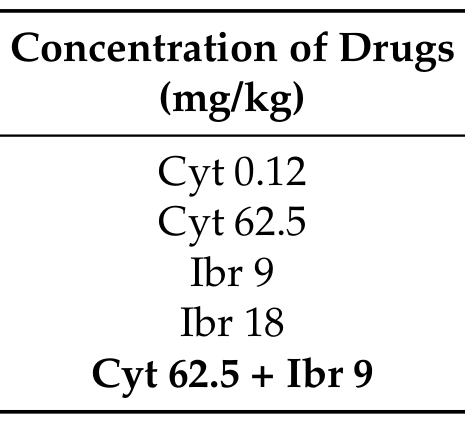
\includegraphics[scale = 0.18] {conc.png}
\end{subfigure}
\begin{subfigure}{0.49\textwidth}
\centering
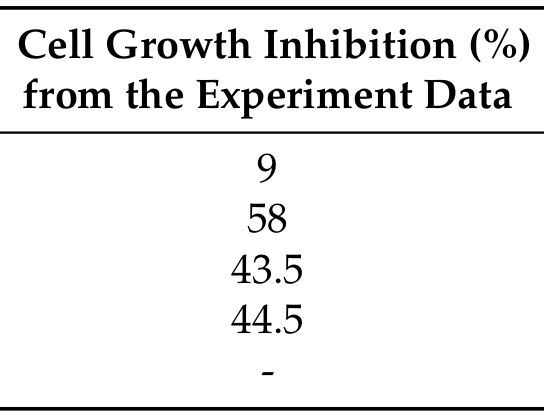
\includegraphics[scale = 0.18] {inhibition.png}
\end{subfigure}
\end{figure}
We notice that growth inhibition due to Cyt was dose dependent, whereas inhibition due to Ibr was not. At this point, a total of 12 deterministic simulations were performed, 3 for each treatment group, using $(A = 5.4 \cdot 10^{4}, E = 2500, C = 0)$ as starting point. In the context of the same treatment group, the simulations set themselves apart for the numerical choice of $\mu_{AC}$: Cyt Low was tested with $\mu_{Ac} = 0.0001$, $\mu_{Ac} = 0.001$ and $\mu_{Ac} = 0.003$. Cyt High was tested with $\mu_{Ac} = 0.005$, $\mu_{Ac} = 0.012$, $\mu_{Ac} = 0.02$. Ibr Low was tested with $\mu_{Ac} = 0.001$, $\mu_{Ac} = 0.0041$, $\mu_{Ac} = 0.005$. Ibr High with $\mu_{Ac} = 0.002$, $\mu_{Ac} = 0.0042$, $\mu_{Ac} = 0.006$. Black lines represent cancer evolution without treatment. The goal was finding, for each treatment protocol, the value for $\mu_{Ac}$, among the one proposed, that gives a \textit{simulated cell growth inhibition percentage} similar for the one obtained from the experiments. 
\begin{figure} [h]
    \centering
    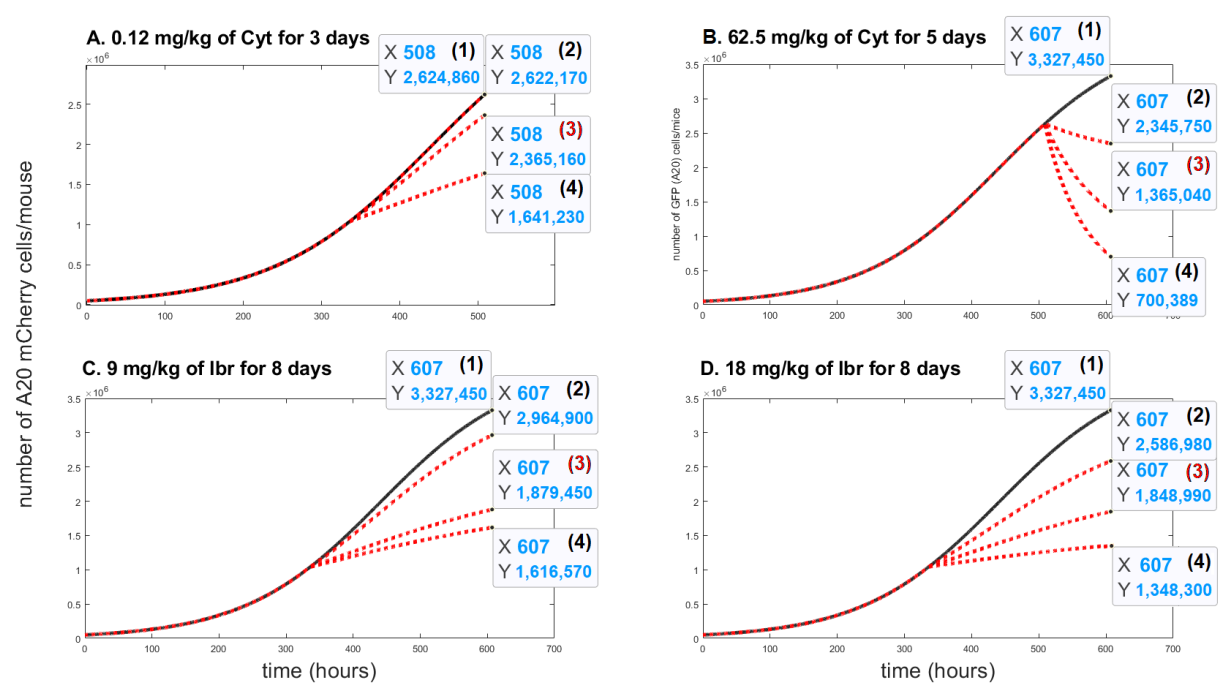
\includegraphics[scale = 0.20] {4.png}
\end{figure}
\begin{itemize}
    \item Cyt Low has a target cell growth inhibition percentage of $9 \%$. This is best reached by using $\mu_{Ac} = 0.001$, that provided $10 \%$ of growth inhibition. 
    \item Cyt High has a target cell growth inhibition percentage of $58 \%$. This is best reached by using $\mu_{Ac} = 0.012$, that provided $59 \%$ of growth inhibition. 
    \item Ibr Low has a target cell growth inhibition percentage of $43.5 \%$. This is best reached by using $\mu_{Ac} = 0.0041$, that provided $43.4 \%$ of growth inhibition. 
    \item Ibr High has a target cell growth inhibition percentage of $44.5 \%$. This is best reached by using $\mu_{Ac} = 0.0042$, that provided $44 \%$ of growth inhibition. 
\end{itemize}
\begin{figure} [h]
    \centering
    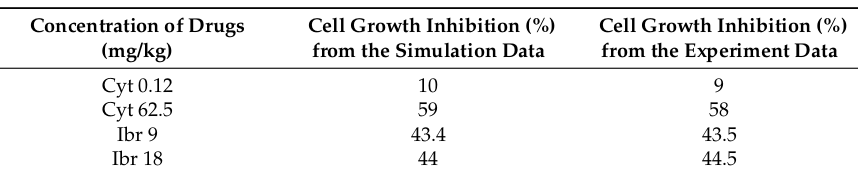
\includegraphics[scale = 0.28] {table.png}
\end{figure}



\subsection{Stochastic approach}
tba


%------------------------------------------------

\section{MATLAB simulations}
\subsection{Code}
The deterministic simulations presented in the paper were replicated by using the MATLAB suite \texttt{ode45}. This library, dedicated to solve systems of differential equations in the form $y'=f(t,y)$, implemnts an adaptive-step Runge-Kutta integration algorithm of the fourth-order. 
We developed the following script to solve the system of equation (1), (2), (3) for each treatment condition.

\begin{lstlisting}

Tf = 1440; % Final time
tspan = [0;Tf];
X0 = [500,2500,0]; % Starting conditions [A(0),E(0),C(0)]
op1 = odeset('MaxStep',1,'RelTol',1e-2,'AbsTol',1e-4);

[t,X] = ode45(@model,tspan,X0,op1);

function dX = model(t,X)

%%% Parameters definition
r = 0.01;   % A20 growth rate [h^-1]
K = 4e6;    % Max A20 number [cells/mouse]
mu_ac = 0.012; % Cyt 62.5 mg/kg for 3 days cytotoxicity rate [h^−1]
mu_ca = mu_ac * 10; % Deactivation of drug due to killing of A20 [h^-1]
d = 1.25 * 2.4e18; % Cyt 62.5 mg/kg dose [molecules/mouse]
mu_c = 0.231; % Cyt chemical deactivation rate [h^-1]
mu_a = 2e-12; % Effectors-A20 interaction coefficient [h^-1]
a = 2e3;    % Drug amount producing 50% of max effect on A20 [molecules]
p = 4e-14; % Production rate of effectors stimulated by A20 [h^-1]
mu_ec = 417; % Mortality rate of drug on effector cells [h^-1]
c = 1e2;    % Num of A20 producing 50% of max immune activation [cells]
b = 5e6;    % Drug amount producing 50% max effect on healty cells [molecules]
mu_ea = 4e-15; % A20-effectors interaction coefficient [h^-1]
mu_e = 4e-5; % Death rate of effecors [h^-1]
tau = 24;

A = r*X(1)*(1-(X(1)/K)) - mu_a*X(1)*X(2) - ((mu_ac*X(1)*X(3))/(a+X(3)));
E = -mu_e*X(2) + (p*X(1)*X(2))/(c+X(1)) - mu_ea*X(1)*X(2)  - (mu_ec*X(2)*X(3))/(b+X(3));
if t(1) > 336 && rem(round(t(1),0),tau) == 0 && t(1) < 384
    C = d - mu_c*X(3) - (mu_ca*X(3)*X(1))/(a+X(1)); 
else
    C = - mu_c*X(3) - (mu_ca*X(3)*X(1))/(a+X(1));
end
dX = [A;E;C];
end

\end{lstlisting}


\subsection{Obtained plots}
\begin{table}[]
\begin{tabular}{|c|c|}
\hline
Group             & Growth Inhibition (\%) \\ \hline
Cyt low           & 70                     \\ \hline
Cyt high          & 11                     \\ \hline
Ibr low           & 45                     \\ \hline
Ibr high          & 44                     \\ \hline
Cyt + Ibr         & 96                     \\ \hline
Cyt infusion low  & 93                     \\ \hline
Cyt infusion high & 98                     \\ \hline
\end{tabular}
\caption{Growth inhibition calculated 2 days after the end of the treatments, with respect to the control group in the same day}
\label{tab:my-table}
\end{table}


%------------------------------------------------
\phantomsection
\section{Conclusions} % The \section*{} command stops section numbering
The goal of the project was to perform a critical examination of the selected publication, focusing in particular on the computational elements. To build a context for the reader, some background information on CLL was provided, together with an outline of modern treatment strategies. More detailed information regarding the two drugs discussed in the paper, Cytarabine and Ibrutinib, were also supplied. \\
The mathematical model was described in all of its terms, and a stability analysis was performed to identify possible equilibrium points and classify their stability. Two biologically feasible equilibria were found: an unstable tumour-free equilibrium $Eq_{0}^{*}$ and an asymptotically stable equilibrium $Eq_{0}^{*}$, in which the number of cancer cells is at carrying capacity. In this condition, if the treatment was stopped and the residual diseases totalled to just a single malignant cell, cancer would still grow back to carrying capacity. This may represent a state of cancer cell dormancy, an adaptive strategy used by cancer cells to overcome drug cytotoxicity. This stage may persist until the complete metabolism of the drug, which would allow tumour growth to recur. \\
The treatment protocols were introduced, together with the experimental parameter estimation employed by the authors of the paper to derive the instantaneous growth rate $r$ and the cytotoxicity rate $\mu_{AC}$. One simulation regarding combined therapy was discussed. \\
Simulations were run to try to reproduce all the protocols listed in the paper. A discrepancy of three orders of magnitude between the dosage reported in the paper and the ones expected from the computations was observed, and it was decided to proceed by using the latter. Despite this, the percentage growth inhibition derived from running the different simulations with the correct protocols were matching the results of the paper in all but one case, that is Cyt High. This discrepancy is probably due to some inconsistency in the paper. An additional discrepancy was observed when trying to reproduce the results of figure A2 in the paper. \\ 
It was derived from the literature that the right administration strategy for Cytarabine is a constant infusion, as opposed to the injection strategy modelled by the third differential equation. Two new mathematical models were built to simulate the first condition, and simulations were run with the treatment protocol derived from paper \cite{cyt-3}. \\
Different additional criticalities were detected: the growth rate $r$ of A20 cells was estimated in immuno-competent Balb/c mice. Therefore, $R$ already carries, implicitly, the contribution of the immune system towards the reduction of the malignant mass. Yet, in the first equation of the mathematical model, there are explicit terms that reproduce the competition with the immunity effector cells, whose dynamics are modelled by the second equation. This redundancy can lead to a dangerous overestimation of the capabilities of the immune system to fight cancerous cells. It was also noticed that the model does not take into account the natural production of effector cells. For this reason, additional simulations were run, implementing an $e_{0}$ term to represent this behaviour. Finally, it was noticed that many parameters used for the drugs and drugs-cancer interactions were taken from a study (referenced with the number 36 in the original paper) that is not concerned with Cytarabine or Ibrutinib, but with Cyclophosphamide. \\
From the growth inhibitions percentages obtained, it was observed that Cyt, a drug not currently used to treat CLL, is more cytotoxic to A20 cells \textit{in vitro} than Ibr, which suggests a repurposing of this cancer drug. A numerical simulation of the potential effect of Cyt plus Ibr on A20 cells, performed in the original paper, predicted that such a combination could increase cytotoxicity and inhibit cancer cell growth by up to 95\%. It would now be valuable to test this combined treatment \textit{in vivo}, especially as these drugs have different modes of action. 

%\addcontentsline{toc}{section}{Conclusions} % Adds this section to the table of contents

%----------------------------------------------------------------------------------------
%	REFERENCE LIST
%----------------------------------------------------------------------------------------
%\newpage
%\phantomsection
\printbibliography
%\bibliographystyle{unsrt}
%\bibliography{bibliography.bib}

%----------------------------------------------------------------------------------------

\end{document}
